
\documentclass[11pt]{article}
\usepackage{acl2014}
\usepackage{times}
\usepackage{url}
\usepackage{latexsym}
\usepackage{graphicx}

\title{CS 288: Parsing}

\author{Anting Shen \\
  23566738 \\
  {\tt antingshen@berkeley.edu} \\
}
\date{October 17, 2014}

\begin{document}
\maketitle

\section{Introduction}
Below are implementations of an unlexicalized PCFG English parser. 
The first being a generative parser, and the second implements 
coarse to fine pruning with a simple grammar.
Lastly, additional optimizations are made based on work in Klein and Manning 03
to further improve F1 scores and computational performance.

\section{Generative Parser}

The generative parser uses a straightforward CKY algorithm. A grammar
(from the provided Grammar class) is generated from annotated
trees and a UnaryClosure class is used to collapse and re-expand chains of unary rules to allow
application of a binary rule at every other step to prevent infinite unary chains. Each unary
step also enforces addition of a reflexive rule to indicate a lack of unary rule at that step.

The tree annotator uses $v=2, h=2$ vertical and horizontal markovization, which showed considerable
F1 improvement over the $v=1, h=\infty$ default, with most of the improvement being from the
switch from $v=1$ to $v=2$, and a smaller improvement from $h=\infty$ to $h=2$.

The CKY tables needed for bottom-up CKY are implemented as three dimensional double arrays, one for
unary and one for binary, and with the array being triangular instead of square to prevent memory
waste. Backpointers are kept in a separate same sized array to save memory of
creating a wrapper object and provide memory locality when performing score lookups. Backpointers
consist of the rule used at that cell, and the split point $k$ for binary rules. Helper functions
recursively reconstruct the tree at the end of parsing, expanding UnaryClosures and ignoring reflexive
rules.

With this implementation on the max length 40 data set, the parser achieves an F1 of 79.0
in 27 minutes on an i5-4670 processor.

\section{Coarse to Fine Parser}

The inside-outside algorithm is used to calculate probabilities of trees in the coarse grammar.
A cell in the fine grammar's table is filled with negative infinity if the corresponding probability
in the coarse grammar is below a threshold. The probability is calculated by
$I(x,i,j)+O(x,i,j)-I(0,0,0)$, where $I$ and $O$ are inside and outside log probabilities, calculated
using max instead of sum as an estimate due to difficulty of summing log probabilities.
To find the corresponding coarse tag from a fine tag, a precomputed indexed mapping array is used.
The coarse grammar is $v=1, h=0$, and its CKY tables are additional multidimensional arrays.

Manual binary search was used to find a balanced threshold between F1 and speed at a log
probability of -7.
The parser achieves on the 40 length set a F1 of 78.53 in 751 seconds on the same processor,
for a 2.16x speed-up.

\section{Additional Optimizations}
This section includes additional exploration and optimizations of both accuracy and performance.
These optimizations are only for the coarse to fine parser and are not back ported to the
generative parser. All tests are performed on the length 40 training and test set.

\subsection{Increasing Vertical Markovization Order}
Klein and Manning 03 suggests that increased vertical order produces better F1, so grandparent
annotations were added to increase $v$ to 3. This increased F1 to 79.93
at a cost of increasing running time to 932 seconds due to a large increase in grammar size.
However, the amount of time did not increase as much relative to the grammar size thanks to
coarse to fine pruning.

\subsection{Collapsing Sparse Grammar Rules}
With increased Markovization order and increased number of grammar rules, many rules have only been
seen a small number of times. Following Klein and Manning, the grammar was modified to only split
rules horizontally if it has been seen at least 10 times. Rules are still always split vertically.
This gives a new Markovization order of $h\leq 2$. With this improvement, F1 increased to 80.0
and the reduced number of grammar rules cut the running time back down to 749 seconds.

\subsection{Additional Annotations}
Many of the remaining mistakes are caused by the grammar using the same tag for different contexts
that should get their own tag. To address this, more annotations are added to produce a finer grammar.
First, the \texttt{UNARY-INTERNAL} mark was added to non-preterminal non-root unary nodes,
which increased F1 to 80.52 and reduced running time to 687 seconds. Adding \texttt{UNARY-RB} and
\texttt{UNARY-DT} further improved F1 to 80.81 and cut time to 634 seconds.

Splitting tags seemed like another possible addition. When \texttt{IN} tags were directly
annotated with their respective words, i.e. lexicalized, F1 increased to 80.93, and time increased to
740 seconds. However, this method splits the \texttt{IN} tag 170 different ways. A better approach
would be to split based on linguistic categories like in Klein and Manning 03,
but the does not explain in detail how \texttt{IN} tags were split. When I experimented with
annotating with case-insensitive words to bring the split down to 97-way, F1 stayed at 80.91
while time increased to 826 seconds. Then I experimented with splitting the words into groups
such as prepositions and subordinating conjuctions, which resulted in a F1 of 80.89 and a time of
683 seconds. The lackluster accuracy gain of tag splitting is most likely due to mistakes in
categorizing the words, and getting better performance would require more linguistics experience.

\subsection{Array Rearrangement}
To improve performance, I experimented with rearranging the tables in memory. Because the loop over
tags is inside the loop over $i$ and $j$, the array should be rearranged as [$i$][$j$][$tag$] instead
of the way presented in the slides to improve memory locality. Furthermore, instead of using a
3D array, the arrays were flattened into one large array since index calculation,
even with a triangular array, takes insignificant time according to a CPU profiler. Flattening the
array and rearranging indexing order decreased the time to 500 seconds. A separate indexing scheme
was then added for outside algorithm, since its array access order differed, to ensure the algorithm
accessed consecutive spots in memory. Additionally, since CKY only reads cells it has filled,
a single large preallocated array is used with no erasing between sentences. All this cut the time down
to 465 seconds.

\subsection{Tuning Pruning Threshold}
One parameter to tune is the probability of the coarse grammar at which
we prune the fine grammar. As expected, F1 increases as we prune less, with 
diminishing returns, and compute time increases as well.
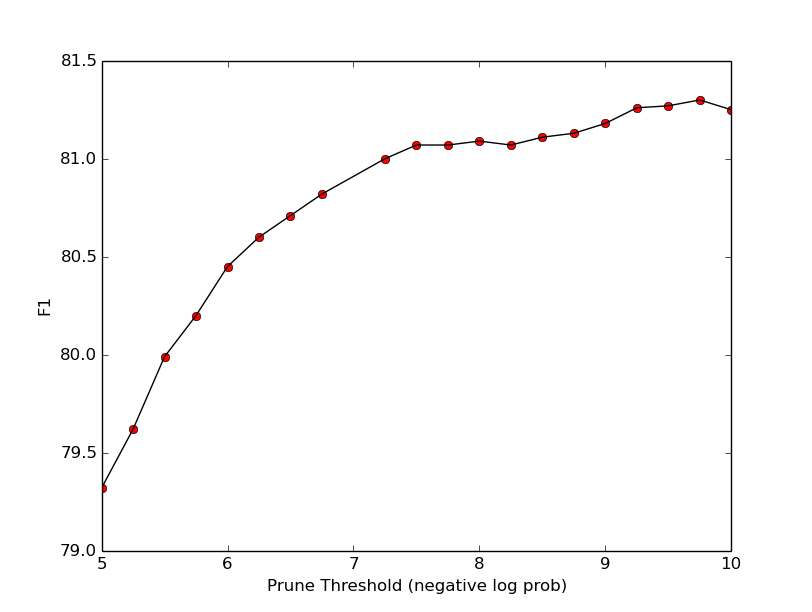
\includegraphics[keepaspectratio=true, width=220px]{thresh_f1.png}
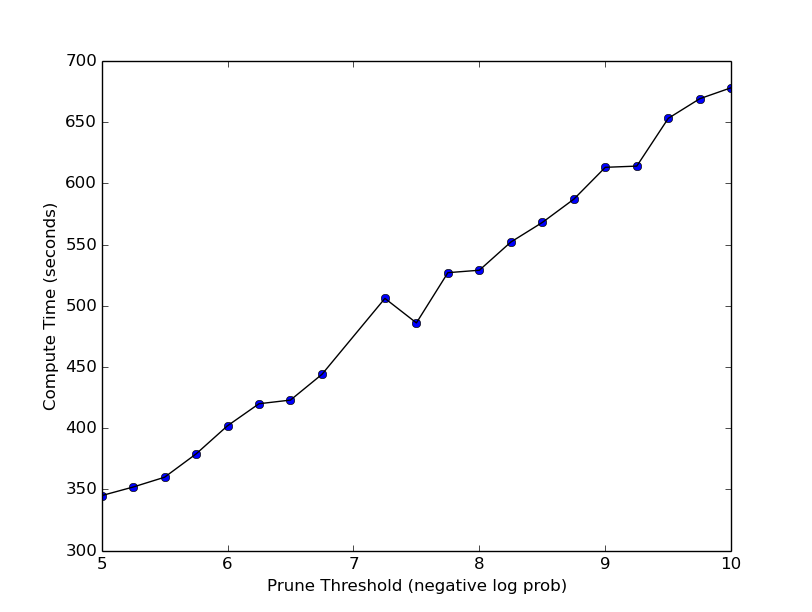
\includegraphics[keepaspectratio=true, width=220px]{thresh_time.png}

Although F1 reaches a peak of 81.3, and reaching 80 F1 required around 6 minutes, 
a compromise between speed and accuracy for the submission was
picked at a threshold of -7.5, with a F1 of 81.07 and a time of 487 seconds. 

\subsection{Other Minor Optimizations}
\begin{itemize}
\item If pruning is too aggressive for a sentence and no tree is found,
the parser is re-run with pruning turned off.
\item In binary rule expansion, if score of one child is already smaller than the current best,
do not check the other child.
\item Similarly, in coarse to fine pruning, if outside score minus denominator is already smaller
than threshold, prune without checking inside score.
\end{itemize}

\section{Final Results}
81.15 F1 in 490 seconds


\end{document}
